\documentclass[10pt,twocolumn,letterpaper]{article}

\usepackage{cvpr}
\usepackage{times}
\usepackage{epsfig}
\usepackage{graphicx}
\usepackage{amsmath}
\usepackage{amssymb}

% Include other packages here, before hyperref.
\usepackage{url}
\usepackage{subfig}
\usepackage{color}

% If you comment hyperref and then uncomment it, you should delete
% egpaper.aux before re-running latex.  (Or just hit 'q' on the first latex
% run, let it finish, and you should be clear).
\usepackage[pagebackref=false,breaklinks=true,colorlinks,bookmarks=false]{hyperref}

% Command definitions
\def\subsectionautorefname{section}
\newcommand{\note}[1]{\textcolor{red}{\textbf{#1}}}
\definecolor{light-gray}{gray}{0.3}
\newcommand{\aside}[1]{\textcolor{light-gray}{\emph{#1}}}
\newcommand{\comment}[1]{}

% \cvprfinalcopy % *** Uncomment this line for the final submission

\def\cvprPaperID{2283} % *** Enter the CVPR Paper ID here
\def\httilde{\mbox{\tt\raisebox{-.5ex}{\symbol{126}}}}

\ifcvprfinal\pagestyle{empty}\fi
\begin{document}

\title{Timely Object Detection}

\author{First Author\\
Institution1\\
Institution1 address\\
{\tt\small firstauthor@i1.org}
% For a paper whose authors are all at the same institution,
% omit the following lines up until the closing ``}''.
% Additional authors and addresses can be added with ``\and'',
% just like the second author.
% To save space, use either the email address or home page, not both
\and
Second Author\\
Institution2\\
First line of institution2 address\\
{\small\url{http://www.author.org/~second}}
}

\maketitle
% \thispagestyle{empty}

\begin{abstract}
In a large, multi-class detection system, the problem of timeliness of results is crucial.
We are motivated by situations where running all detectors would take an unacceptably long time, and the best answer must be given by some deadline.
Our system for multi-class detection aims to give the best possible results at any single point after a start time; it is terminated at a deadline time.
Toward this goal, we formulate a dynamic policy to decide which detector to deploy next.
The policy is guided by an estimate of the contents of the image, and is sensitive to the time deadline and the ``value'' of different classes.
We evaluate parametrizations of the policy with respect to performance in the novel AP vs. Time evaluation on the PASCAL VOC dataset.
\end{abstract}

%!TEX root=paper/paper.tex
\chapter{Introduction}\label{sec:introduction}

\section{Motivation}

\PM{Perception}
It is well-known that human perception is Anytime, meaning that a scene can be described after even a short presentation.
Perception is also progressive, meaning that the quality of description increases with more time.
The progressive time course of visual perception has been confirmed by multiple studies \parencite{Vanrullen-1996,Fei-Fei-Vision-2007}, with some studies providing evidence that enhancement occurs in an ontologically meaningful way.
For example, people tend to recognize something as an animal before recognizing it as a dog \parencite{Mace-PloS-2009}.
The underlying mechanisms of this behavior are unknown, and only a few attempts have been made to explain the temporal dynamics (for instance, a promising work by \cite{Hegde-Neuro-2008} has employed the framework of sequential decision processes).

\PM{Computer applications}
Meanwhile, automated visual recognition has achieved levels of performance that allow useful real-world implementation.
We focus on two problem formulations: \emph{image classification}, in which some property of the image -- such as scene type, visual style, or even object presence -- is predicted, and \emph{object detection}, in which the location and category (or identity) of all objects in a scene is predicted.
Solutions to the two problems are often linked, as classification can be a subroutine for detection.
Our motivation is that state-of-the-art methods for classification and detection tend to be computationally expensive, insensitive to Anytime demands, and not progressively enhanced.

\PM{Application}
As real-world deployment of recognition methods grows, managing resource cost (power or compute time) becomes increasingly important.
For tasks such as personal robotics, it is crucial to be able to deploy varying levels of processing to different stimuli, depending on computational demands on the robot.
A hypothetical system for vision-based advertising, in which paying customers engage with the system to have their products detected in images on the internet, presents another example.
The system has different values (in terms of cost per click) and accuracies for different classes of objects, and the backlog of unprocessed images fluctuates based on demand and available server time.
The recognition strategy to maximize profit in such an environment should exploit all signals available to it, and the quality of detections should be Anytime, depending on the length of the queue (for example, lowering recall when queue pressure grows).

\PM{Visual Features / Classification}
For most state-of-the-art classification methods, a range of features are extracted from an image instance and used to train a classifier.
Since the feature vectors are usually very high-dimensional, linear classification methods are used most often -- for instance, logistic regression.
Features are extracted at different costs, and contribute differently to decreasing classification error.
Although it can generally be said that ``the more features, the better,'' high accuracy can of course be achieved with only a small subset of features for some instances.
Additionally, different instances benefit from different subsets of features.
For example, simple binary features are sufficient to quickly detect faces \parencite{Viola-IJCV-2004} but not more varied visual objects, while the features most useful for separating landscapes from indoor scenes \parencite{Xiao-CVPR-2010} are different from those most useful for recognizing fine distinctions between bird species \parencite{Farrell-ICCV-2011}.
\autoref{fig:features} presents several common visual features.

\PM{Detection}
Detection methods tend to employ the same visual features and classifiers but apply them to many image sub-regions.
Approaches can broadly be grouped into \emph{per-class, exhaustive-region}, \emph{all-class, exhaustive-region}, and \emph{all-class, proposed-region} methods.
State-of-the-art \emph{per-class, exhaustive-region} methods such as \cite{Felzenszwalb2010a} and \emph{all-class, proposed-region} methods such as \cite{Girshick-CVPR-2014} are considerably slow, performing an expensive computation on a thousand to a million image windows.
To maximize early performance gains of these methods, scene and inter-object contextual cues can be exploited in two ways.
First, regions can be processed in an intelligent order, with most likely locations selected first.
Second, if detectors are applied per class, then they can be sequenced so as to maximize the chance of finding objects actually present in the image.
And even the most recent \emph{all-class, exhaustive-region}, Convolutional Neural Net (CNN)-based detection methods such as \cite{He-ECCV-2014}, which take advantage of high-performance convolutional primitives for region processing and detect for all classes simultaneously, can be sped up using Anytime ideas such as cascaded classification.

\section{Our Work}

\PM{Costliness}
Computing all features, running all detectors, or processing all regions for all images is infeasible in a deployment sensitive to Anytime needs, as each feature brings a significant computational burden.
Yet the conventional approach to evaluating visual recognition does not consider efficiency, and evaluates performance independently across classes.
We address the problem of selecting and combining a subset of features under an Anytime cost budget, specified in terms of wall time or total power expended or another metric, and propose a new \emph{costliness} measure of performance vs. cost.

\PM{Learning a Policy}
To exploit the fact that different instances benefit from different subsets of features, our approach to feature selection is a sequential policy.
To learn the policy parameters, we formulate the problem as a Markov Decision Process (MDP) and use reinforcement learning methods.
The method does not make many assumptions about the underlying actions, which can be existing object detectors and feature-specific classifiers.
With different settings of parameters, we can learn policies ranging from \textbf{Static, Myopic}---greedy selection not relying on any observed feature values, to \textbf{Dynamic, Non-myopic}---relying on observed values and considering future actions.
The foundational machinery is laid out in \autoref{sec:det_method}.

\PM{Per-class Detection}
For \emph{per-class} detection, the actions are time-consuming detectors applied to the whole image, as well as a quick scene classifier.
We run scene context and object class detectors over the whole image sequentially, using the results of detection obtained so far to select the next actions.
Since the actions are time-consuming, we use a powerful inference mechanism to select the best next action.
In \autoref{sec:det_evaluation}, we evaluate on the PASCAL VOC dataset and obtain better performance than all baselines when there is less time available than is needed to exhaustively run all detectors.

\PM{Image Classification}
Classification actions are much faster than detectors, and the action-selection method accordingly needs to be fast.
Because different features can be selected for different instances, and because our system may be called upon to give an answer at any point during its execution, the feature combination method needs to be robust to a large number of different observed-feature subsets.
In \autoref{sec:clf_chapter}, we consider several value-imputation methods and present a method for learning several classifiers for different clusters of observed-feature subsets.
We first demonstrate on synthetic data that our algorithm learns to pick features most useful for the specific test instance.
We demonstrate the advantage of non-myopic over greedy, and of dynamic over static on this and the Scene-15 visual classification dataset.
Then we show results on a subset of the hierarchical ImageNet dataset, where we additionally learn to provide the most specific answers for any desired cost budget and accuracy level.

\PM{Cascaded CNN}
We additionally investigate a novel approach for speeding up a state-of-the-art CNN-based detection method, and propose a general technique for accelerating CNNs applied to class imbalanced data.
We bring the classic idea of the cascade to CNNs by inserting a \emph{reject} option between CNN layers.
When the CNN processes batches of images, which is standard for many applications, the reject layers allows the CNN to ``thin'' the batch as it progresses through the network, thus saving processing time.
This method is applicable to both \emph{all-class, proposed-region} methods such as \cite{Girshick-CVPR-2014} and \emph{all-class, exhaustive-region} methods such as \cite{He-ECCV-2014}.
We demonstrate results --- along with a variety of strong baselines -- on the former method, and show that the Cascaded CNN method obtains a nearly 10x speed-up with only marginal drop in accuracy.
All work is reported in \autoref{sec:ccnn_chapter}.

\PM{Recognizing Style}
Lastly, in \autoref{sec:style_chapter}, we present two novel datasets and first results for an underexplored research problem in computer vision -- recognizing visual style.
In preparation for an Anytime approach, we evaluate several different features (including CNNs) for the task, and explore content-style correlations in our datasets.
Our large-scale learning gives state-of-the-art results on an existing dataset of image quality and photographic style, and provides a strong baseline on our contributed datasets of 80K photos and 85K paintings labeled with their style and genre.
In a demonstration of cross-dataset understanding of style, we show how results of a search by content can be filtered by style.

\PM{Future Directions}
This works provides an effective foundation for further exploration of Anytime recognition, and points the way to interesting further development.
Our MDP-based formulation of learning a feature-selection policy is empirically effective, but heuristic in nature.
The recently developed framework of adaptive submodularity \parencite{Golovin-and-Krause-2010-JAIR} could provide theoretical near-optimality results for some policies, but developing an appropriate objective for our task is not straightforward.
We showed our Cascaded CNN model to be effective for a region-based detection task -- but the model was not trained end-to-end with the threshold layers.
An even more interesting future development would add an Anyitme loss layer that combines classification output from multiple levels of the network in a cost-sensitive way.
We explain these ideas in detail in \autoref{sec:conclusion}.
 % includes Evaluation section
% !TEX root = paper/paper.tex
\section{Related Work}
% \paragraph{Feature combination and selection.}
% \emph{Boosting} is a method for combining weak learners into a more powerful classifier \cite{Hastie2009}.
% A popular use of boosting is in introducing non-linearities by training depth-limited decision trees as weak learners---the boosting trick.
% For SVM-based classifiers, \emph{Multiple Kernel Learning} (MKL) provides a way to train classifiers using an automatically weighted combination of kernels \cite{Lanckriet2004}.
% It has been shown that MKL is outperformed by boosting single-kernel classifiers \cite{Gehler2009}.
% Of course, if all classifiers are linear, then combining outputs of classifiers trained on different feature channel with another classifier is equivalent to training one classifier on all features at once.
% \todo{What about learning a \emph{non-linear} second classifier on top of the weak learner scores---any papers?}

% \todo{A couple of sentences on feature selection approaches, particularly using infogain as proxy for classification error.}

\paragraph{Static selection}% test-time efficient feature selection.}
% The simplest way to limit the number of features used at test time is to $L_1$-regularize.
% This method does not explicitly consider feature cost, nor is it able to evaluate features one by one, or to give an answer before all features are computed.

A well-known method to evaluate features sequentially is the cascaded boosted classifier of Viola \& Jones \cite{Viola2004} (updated by Bourdev \& Brandt \cite{Bourdev-CVPR-2005} with a soft threshold), which is able to quit evaluating an instance before all features are computed---but feature cost was not considered.
The cost-sensitive cascade of Chen et al.\ \cite{Chen-AISTATS-2012} optimizes stage order and thresholds to jointly minimize classification error and feature computation cost.
Xu et al.\ \cite{Xu-ICML-2012} and Grubb \& Bagnell \cite{Grubb-AISTATS-2012} separately develop a variant of gradient boosting for training cost-sensitive classifiers; the latter prove near-optimality of their greedy algorithm with submodularity results.
Their methods are tightly coupled to the stage-wise regression algorithm.

\vspace{-1em}
\paragraph{Dynamic selection}% test-time efficient feature selection.}
The above methods learn an efficient but \emph{fixed} order for evaluating features given a test instance.

Gao \& Koller \cite{Gao-NIPS-2011} propose a method for \emph{active classification}: myopically selecting the next feature based on expected information gain given the values of the already selected features.
The method is based on locally weighted regression, highly costly at test time.
Ji \& Carin \cite{Ji-PR-2007} also formulate cost-sensitive feature selection generatively, as an HMM conditioned on actions, but select actions myopically, again at signficant test time cost.

Karayev at al.\ \cite{Karayev-NIPS-2012} propose a reinforcement learning approach for selecting object detectors; they rely on expensive test-time inference in a graphical model to combine observations.
Dulac-Arnold et al.\ \cite{Dulac-Arnold-ML-2012} present another MDP-based solution to ``datum-wise classification'', with an action space comprised of all features and labels, recently extended to region-based processing \cite{Dulac-Arnold-ICLR-2014}.
He He et al.\ \cite{HeHe-ICMLW-2012} also formulate an MDP with features and a single classification step as actions, but solve it via imitation learning of a greedy policy.
Benbouzid et al.\ \cite{Benbouzid-ICML-2012} formulate an MDP that simply extends the traditional sequential boosted classifier with an additional \emph{skip} action, significantly limiting the space of learnable policies (\cite{Trapeznikov} provides another variation on this problem).
Although \cite{Karayev-NIPS-2012} targets \emph{Anytime} performance, their inference procedure is prohibitively expensive for test-time use in a general classification task.
In contrast, our fast linear method allows direct specification of the Anytime cost budget.

\emph{Label trees} also guide an instance through a tree of classifiers; their structure is determined by the confusion matrix or learned jointly with weights \cite{Deng-NIPS-2011}.
Xu et al.\ \cite{Xu-ICML-2013} learn a cost-sensitive binary tree of weak learners using an approach similar to the cyclic optimization of \cite{Chen-AISTATS-2012}.
Less directly related---but exciting for its novelty---is the work of \cite{weiss2013dynamic}, who apply simple introspection to structured models for a significant speedup of human pose estimation.
Another exciting direction is theoretical analysis of near-optimal policies with humans in the loop \cite{chen14active}.

\section{Multi-class detection policy}
We present a system that deploys multiple detectors to localize all object instances in the image.
The detectors are considered black boxes to the system, but it can measure the statistics of their performance at training time.

Our evaluation approach is explained in more details in Section \ref{sec:evaluation}; here we briefly summarize:
\begin{itemize}
\item The performance of the system is evaluated in the multi-class setting, meaning that detected boxes of a given class are matched to ground truth boxes of all classes, with the corresponding additional capacity for false positives.
\item The underlying performance metric is Average Precision: the area under the Precision vs. Recall curve.
\item Running a detector takes time and generates a list of detections, which are added to all current detections and thus generate a new AP point.
\item The system receives a start time and deadline; we seek to maximize the area under the AP vs. Time curve between these times.
\end{itemize}

Because the system must deliver results on a time budget, the policy must dynamically decide which detector in its arsenal to deploy next.
A symbolic explanation of the policy operation is shown in Figure \ref{fig:pomdp}.
To leverage the signal present in inter-object context, the decision of which detector to run next should be based on the observed results of detector actions that have already been run.
Of course, the observed results of detector actions do not give full confidence to the presence of a class in the image, necessitating an intermediate step from detection statistics to class presence in our system.

First, we look at how to construct such a system with only one detector per class.
We explain the general partially-observable decision process that we face and our choices for the different modular components of it.
We evaluate different ways of obtaining probabilities of object presence, and of estimating the value of running actions.
Next, we generalize the system to be able to handle multiple detector types per class, and show results on this task.

\section{Policy with a single detector per class}
The structure of the problem may be further defined as follows.
There are $|A|$ actions $a_i$.
Although we relax this later, at first we assume that each action consists in running a detector, and so generates a (possibly empty) list of detections when taken.
The same action will always generate the same list of detections, so there is no reason to ever take the same action more than once.

\begin{figure}[htb!]
  \centering
    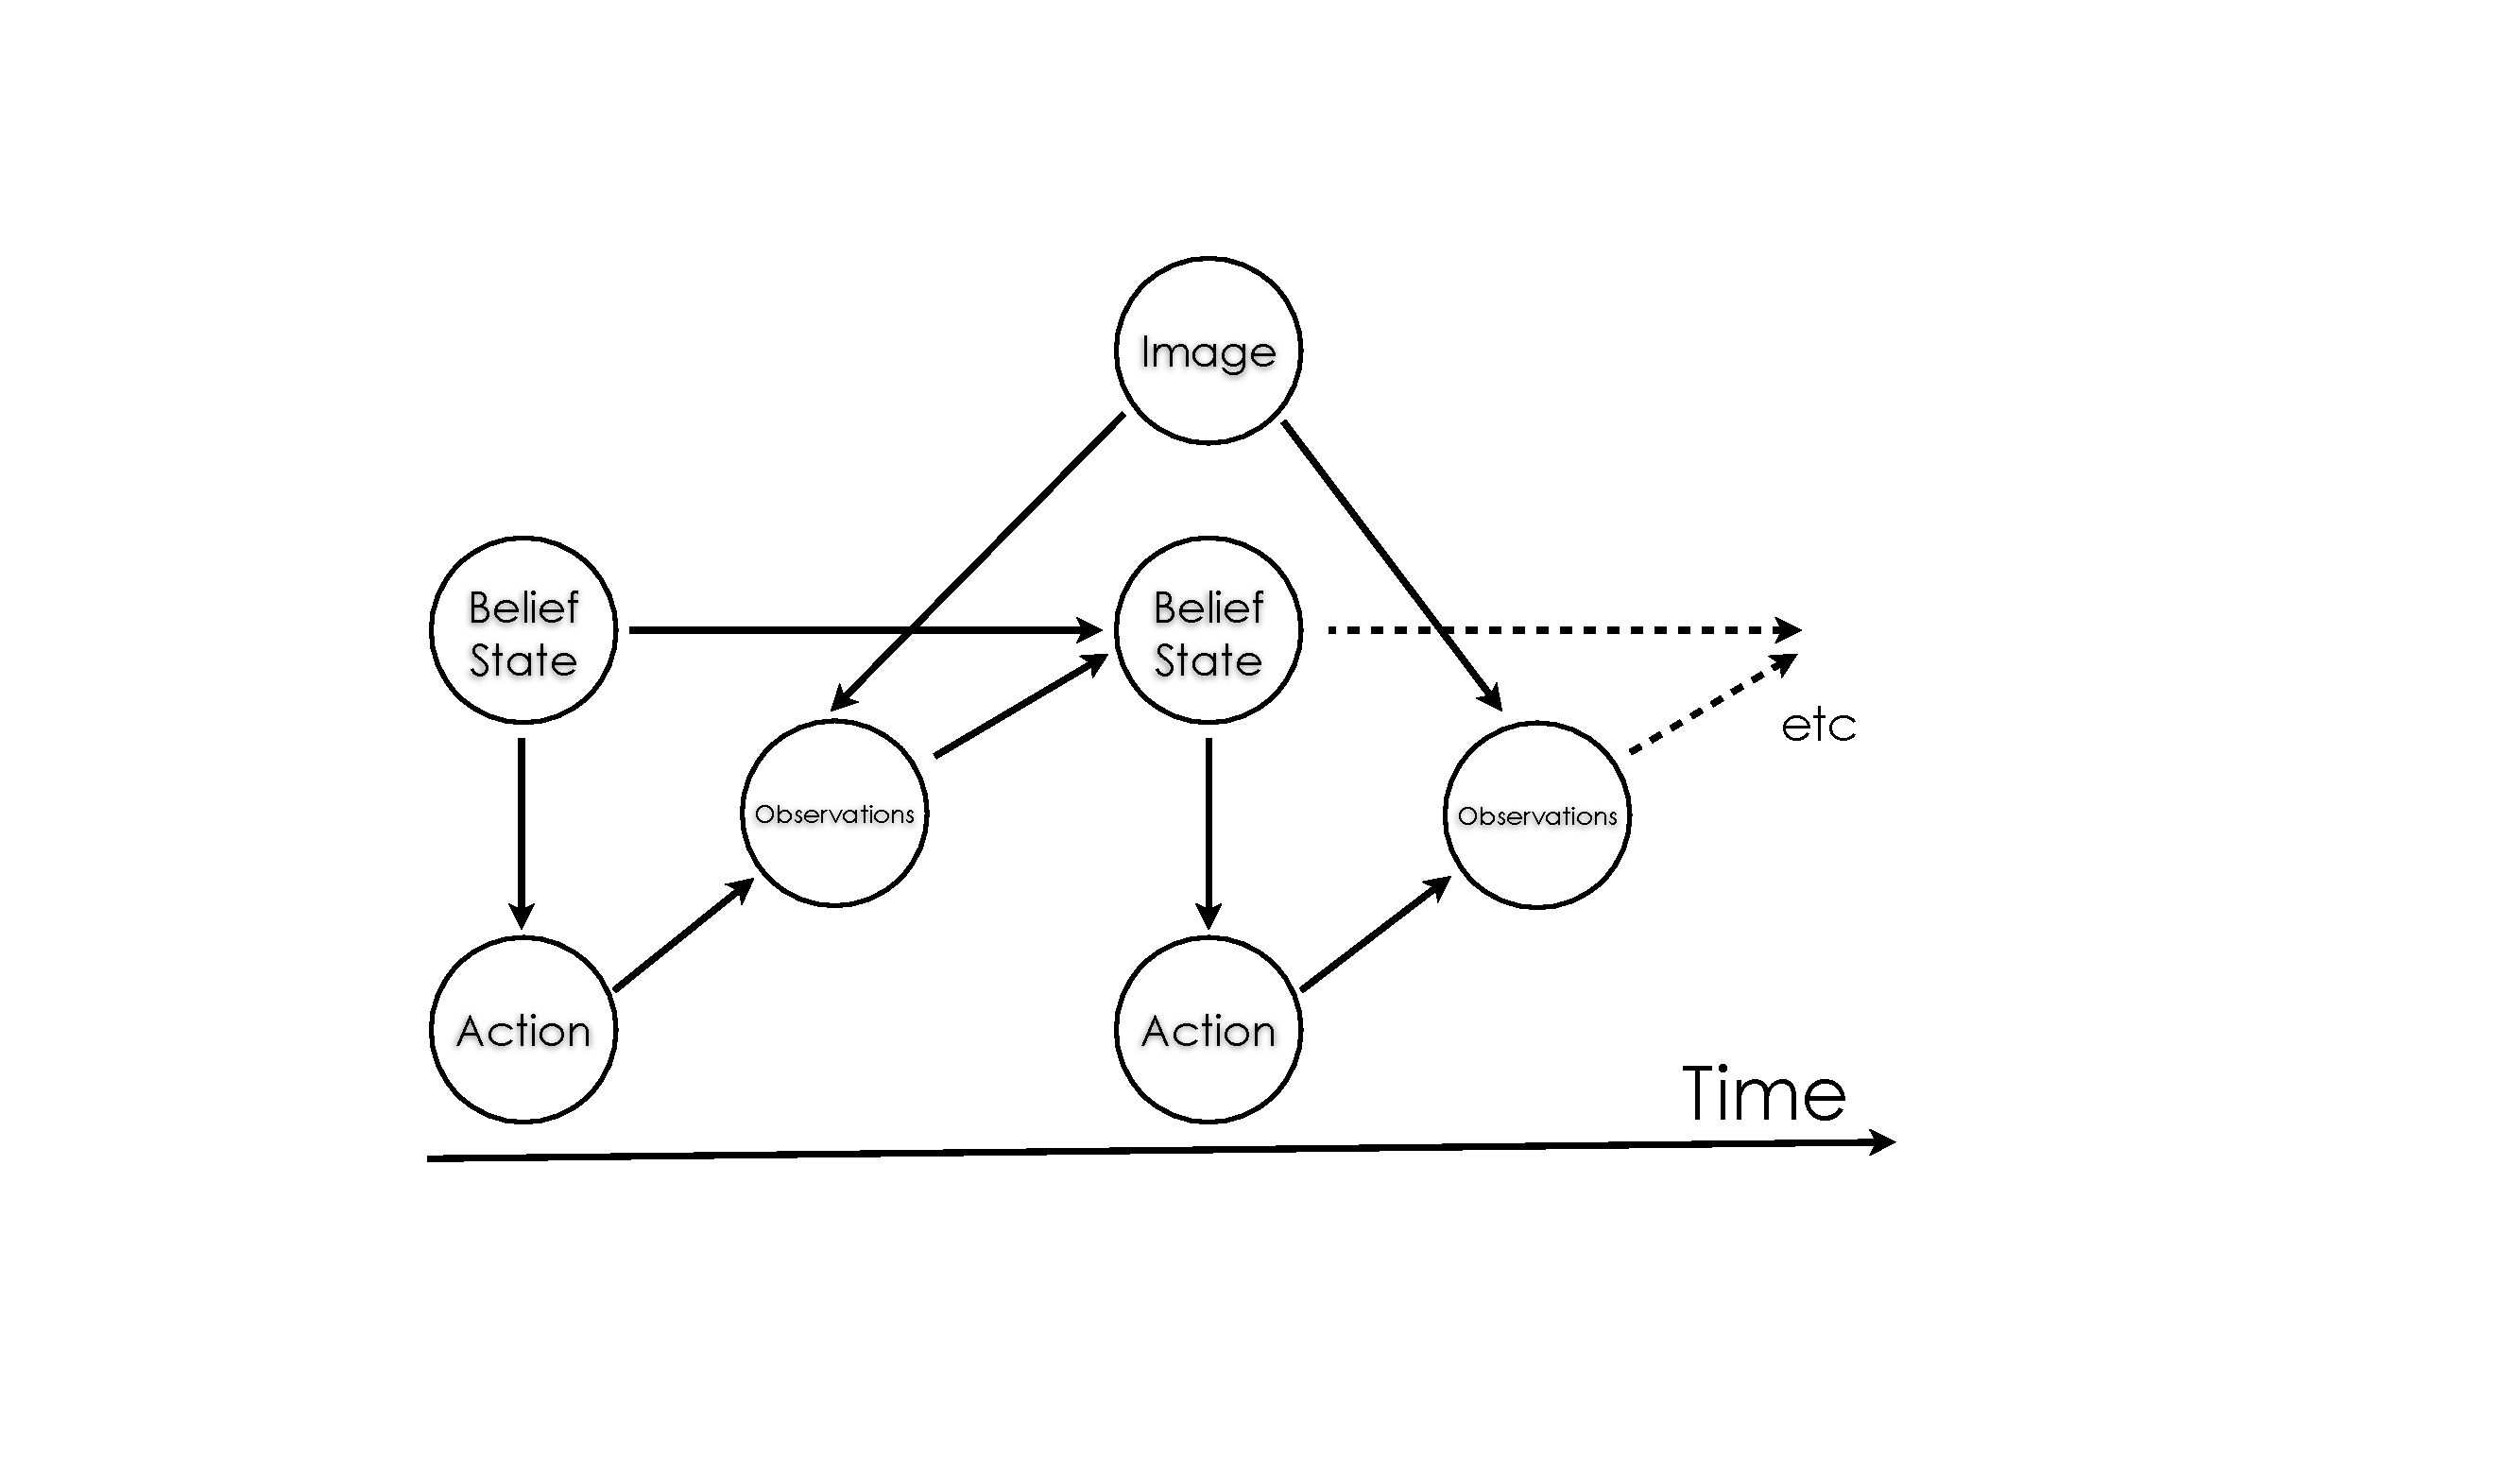
\includegraphics[width=0.9\linewidth]{../figures/pomdp.pdf}
  \caption{Summary of our approach to the problem. Our model consists of two modular parts: predicting the value of taking an action, and updating the latent belief representation having taken an action.}
  \label{fig:pomdp}
\end{figure}

Furthermore, for now we assume that $|A|=K$, the number of target classes in the dataset, so that there is exactly one detector that we can run per class.
The operation of the system, as shown in Figure~\ref{fig:pomdp}, consists in
\begin{enumerate}
\item Selecting which action to take, based on the current estimate of the image contents;
\item Updating the estimate based on the observed detections upon taking the action.
\end{enumerate}

Additionally, after every detection-generating action, the performance of the system is re-evaluated by computing the multi-class Average Precision of the updated list of detections.
This result is not observable by the policy.

We first cover the second modular part of the system: updating the latent belief representation, having already taken an action and received a list of detections.

\subsection{Belief state model}
In the terminology of partially observable decision processes, we call the part of our system that tracks progress the \emph{belief state}.
The belief state maintains inferred probabilities of object presence in the image for all classes; record of the actions taken and the composite list of resulting detections; and the current time into the episode.

In order to exploit the signal due to interobject context, we would like the object presence model to be able to model co-occurrences between object classes.
That is, if through detecting for the class 'person' we become reasonably certain that there indeed is a person in the image, this should boost the expected value of detecting for classes that tend to co-occur with 'person' in the dataset, such as 'motorcycle' or 'horse.'

The co-occurence relations between presences of all the object classes form a highly connected graph of binary random variables $C_i$, $1 \leq i \leq K$.
$C_i = 1$ if there is at least one object of class $K_i$ in the image; otherwise it is $0$.
To infer the value of each binary random variable, we use the list of detections output by a given detector.
In this paper we implement a fast, two-stage approximation to inference in this model.

We use the empirical counts of our training set to formulate initial priors of class presence, such that $P(C_i=1)$, which we write as just $P(C_i)$ for brevity, refers to the number of times class $K_i$ occurs in an image divided by the total number of images in the dataset, and $P(C_i, C_j)$ refers to the similarly normalized number of times classes $K_i$ and $K_j$ occur together in the same image.

Let's say we have inferred values $c_J$ of random variables $C_J$ where $J$ is a set of class indices.
\[
%P(C_i|C_J=c_J)=\frac
%{\sum_{c_K, K \backslash J} P(C_i, C_J=c_J | C_K=c_k)}
%{\sum_{c_K, K \backslash J} P(C_J=c_J | C_K=c_k)}
P(C_i|C_J=c_J)=\frac
{P(C_i, C_J=c_J)}
{P(C_J=c_J)}
\]

If during test time we observe a new setting of objects presences, as is likely to happen quite frequently, using empirical counts will report a probability of $0$.
Accordingly, we need to incorporate some method of smoothing the distribution over all possible assignments.

Our choice is to ``back off'' to a conditional with fewer assignments.
The complete way to do this would be to incorporate all $2^{K-1}$ conditionals of $C_i$  given any subset of the $K-1$ observed variables.
A faster approximation of the conditional is to write it out as follows:
\begin{align*}
P_{back}(C_1 | C_2\ldots C_k) = \frac{P(C_1 , C_2\ldots C_k) }{P(C_2\ldots C_k)} \\
+ \frac{\lambda_1}{K-1} \left(\sum_{i=2}^K P(C_1|C_i) \right) + \lambda_2 P(C_1)
\end{align*}

This model has three terms: the first does not assume any independeces, and relies fully on data; the second assumes the naive Bayes independence of $C_1$ and $C_i$ given any $C_j$, $i\neq j$; the third assumes that there are no dependencies between any $C_i$.
We refer to this model as \textbf{backoff}.

The model \textit{fixed policy} ignores any conditionals and just chooses the next action according to the priors of the single class:
\begin{equation*}
P_{fix}(P_1|P_2\ldots P_k) = P(C_1)
\end{equation*}

Both object class presence probability models are evaluated in Section \ref{sec:actual-evaluation}.

With a set of actions $\mathcal{A}$, progress through the belief states works as follows, starting with belief state $\mathcal{B}_0 = \emptyset$:
\begin{enumerate}
 \item Choose an action $\alpha_i \in \mathcal{A}_i$ that maximizes the value function given $\mathcal{B}_0$.
 \item Execute $\alpha_i$, receiving detections $\beta_i$. 
 \item Update the current assignments to $C_i$ with the new detections $\beta_i$.
 Update $\mathcal{B}_{i+1}$ with the new $C_i$ and the time spent on the action;
 $\mathcal{A}_{i+1} = \mathcal{A}_i\backslash \alpha_i$
 \item Repeat while $\mathcal{A}_{i+1}\neq \emptyset$ and there is time left.
\end{enumerate}
We now provide further explanation of step 3.

\subsection{Inferring $C_i$ from detections}
After executing an action, we get a set of detections: a list of bounding boxes and associated confidence scores for the given class.
We want to infer the presence of at least one object of the class in the image.
Instead of simply tresholding the scores of these detection, we extract a feature vector and classify it with an SVM.
The feature vector consists of a histogram of the values of scores and the count of detections; the parameters of the histogram are selected through cross-validation.
The featurization instead of thresholding helps in cases with no overwhelmingly confident detection, but a large number of detections nevertheless.

Table~\ref{tab:scoreClassifier} shows the performance of our classifiers for the classes of the PASCAL VOC 2007 and the two detectors used in our multiple detector system explained in Section \ref{sec:multidetector}.
We use the metric of accuracy: the number of correct decisions versus the total number of decisions.
\textit{detector} shows the results of the histogrammed CSC-classifier and \textit{detector-fast} is CSC with parameters settings to speed it up to about half the time.

\begin{table}
  \begin{center}
    \begin{tabular}{ c| c c c}
      Class & Detector & Detector-fast\\
      \hline
      aeroplane & 0.7427 & 0.5669\\
      bicycle &  0.8249 & 0.7342\\
      bird & 0.5747 & 0.5565\\
      boat &  0.6935 & 0.6565\\
      bottle  & 0.7027 & 0.6276\\
      bus &  0.5 & 0.7533\\
      car &  0.8565 & 0.7448\\
      cat & 0.6678 & 0.6213\\
      chair  & 0.7029 & 0.5\\
      cow &  0.7160 & 0.6928\\
      diningtable  & 0.6639 & 0.6393\\
      dog  & 0.5520 & 0.5281\\
      horse  & 0.8492 & 0.7077\\
      motorbike  & 0.7588 & 0.7117\\
      person &  0.8063 & 0.7263\\
      %\vdots&\vdots&\vdots&\vdots \\
      pottedplant  & 0.6213 & 0.6115\\ 
      sheep &  0.6978 & 0.6336\\ 
      sofa &  0.6803 & 0.5901\\ 
      train  &  0.8163 & 0.7149\\ 
      tvmonitor & 0.7622 & 0.7066
    \end{tabular}
    \caption{Per-class accuracies of the object presence classifier. Input is a set of detections on an image, output by either the baseline or the \emph{fast} detector.}
    \label{tab:scoreClassifier}
  \end{center}
\end{table}




\subsection{Value Function and the Definition of Rewards}
Having updated the belief state, the system must again pick the next action.
Remember that our system aims to maximize the single-number metric of the area under the AP vs. Time curve.
Accordingly, we define the final reward accrued by a policy to be precisely the area under the curve between start and deadline times.

\begin{figure}[htb]
  \center{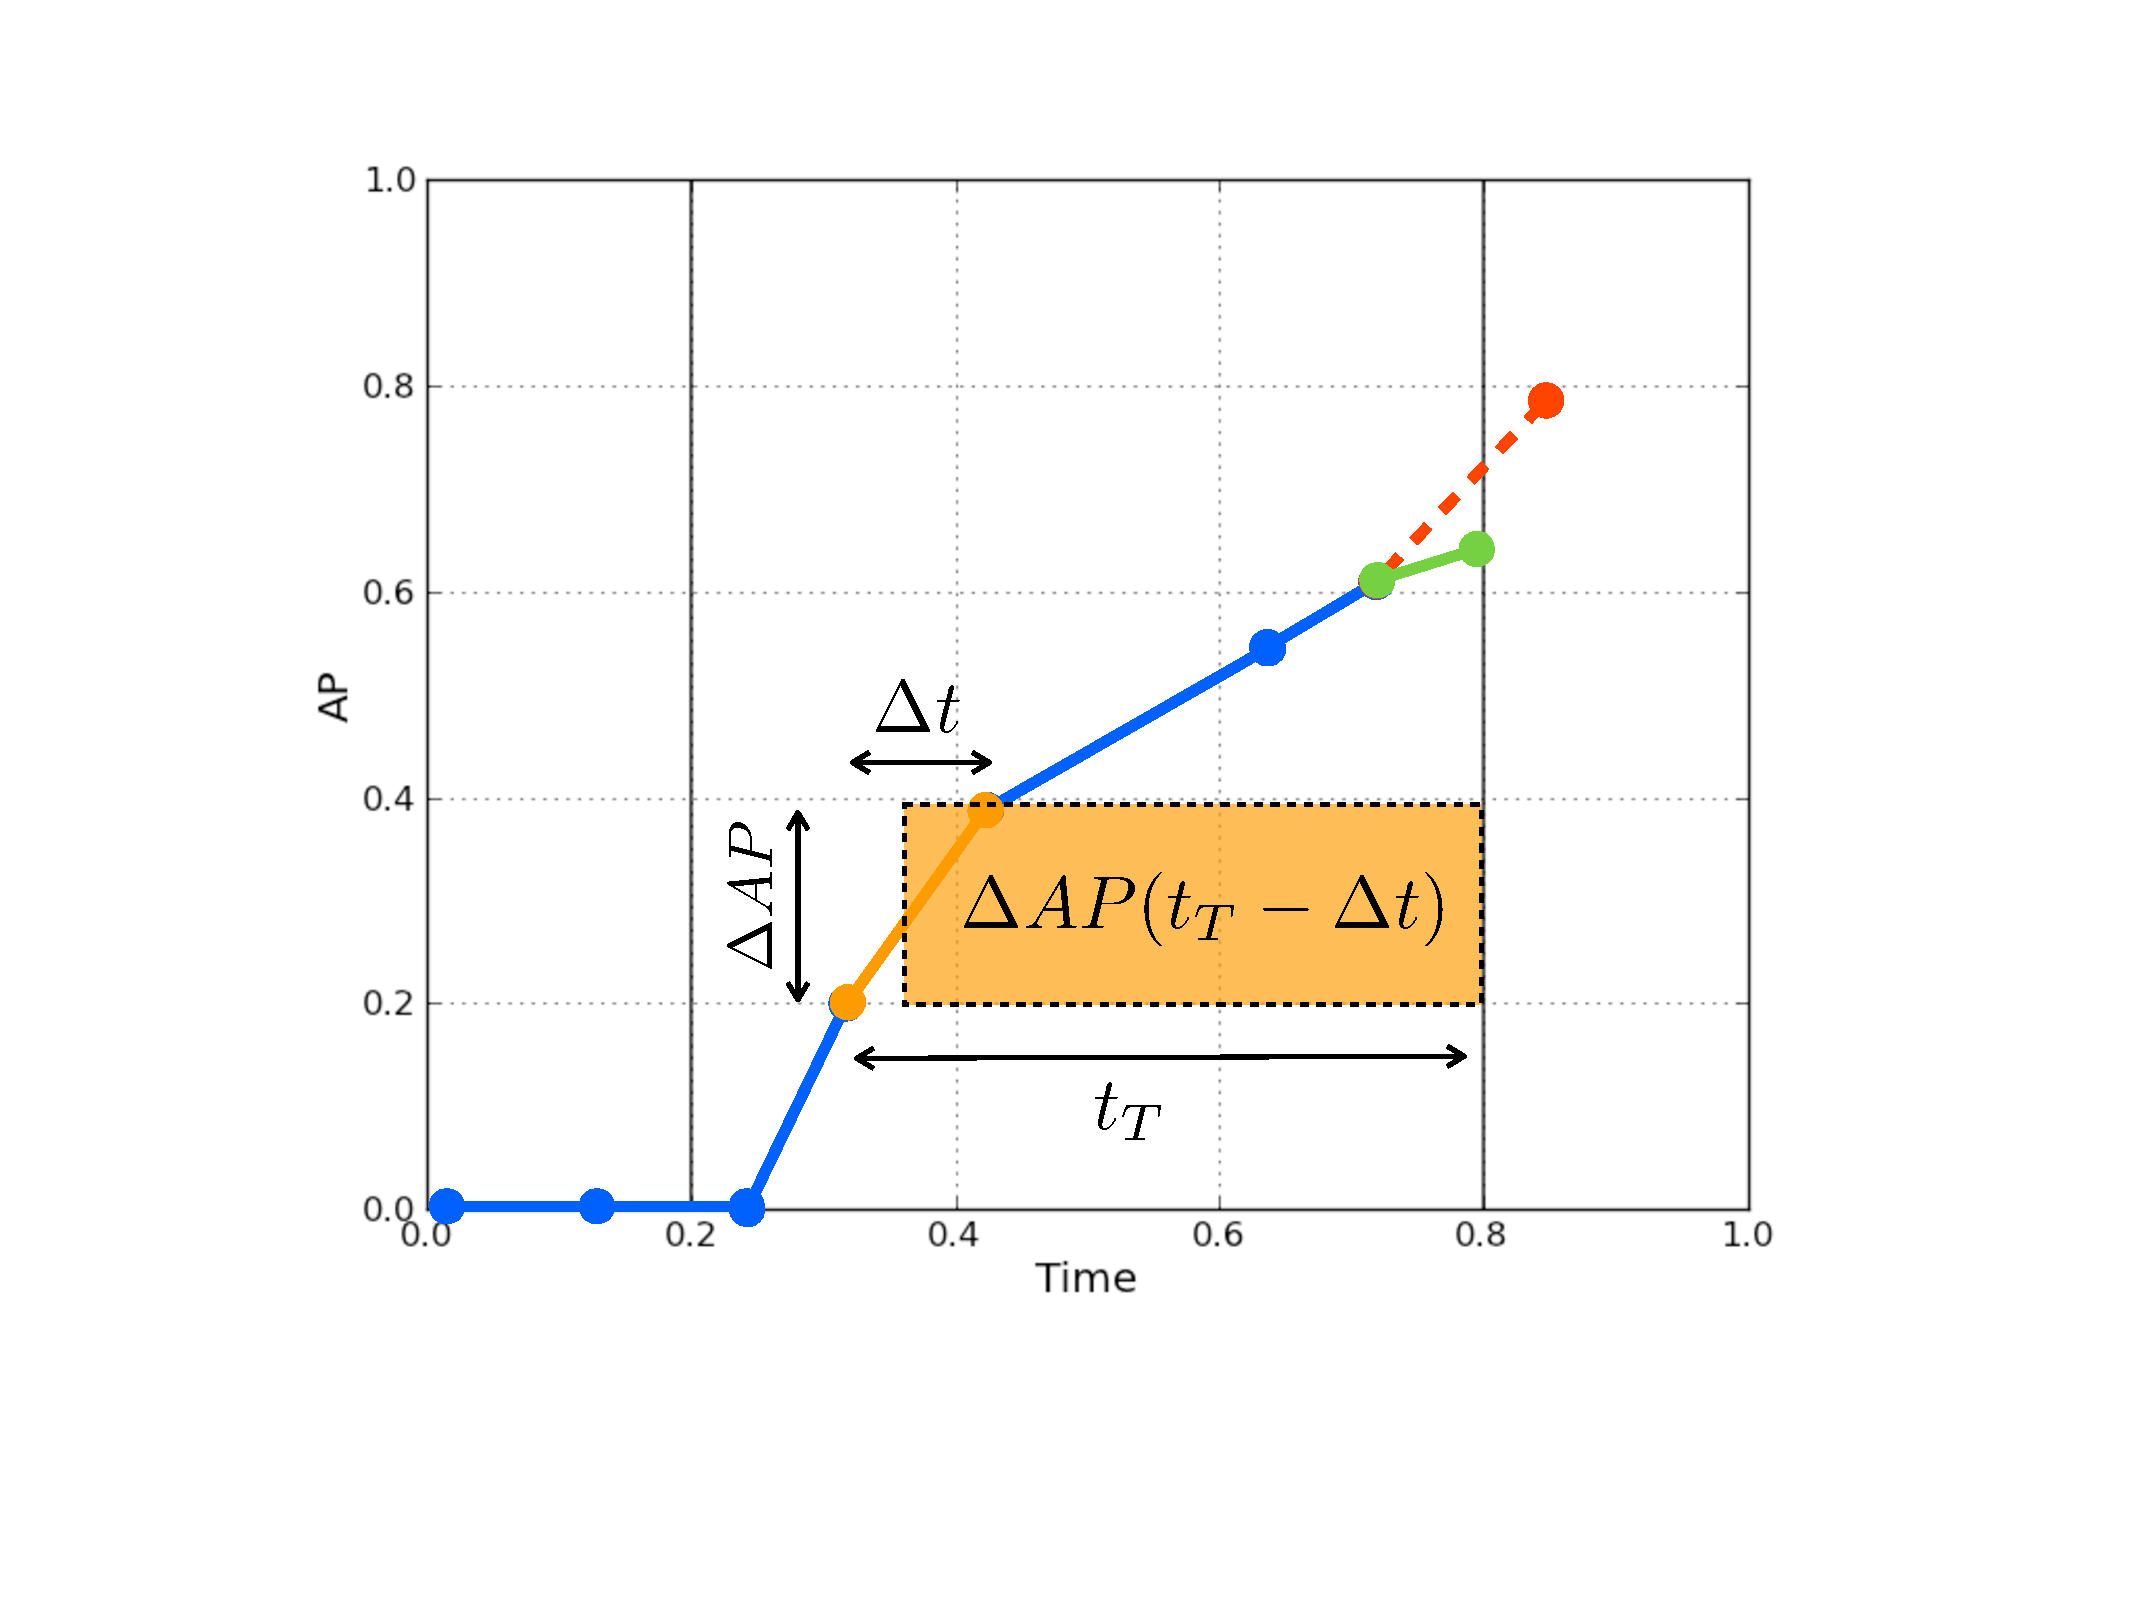
\includegraphics[width=1\linewidth]{figures/apvst_expl.pdf}}
  \caption{\label{fig:rewards}A per-action greedy value function that corresponds to the maximization of our objective function is the ratio of the area of the horizontal slice under the curve due to the action to the maximum possible area the action could have captured. The figure shows this analysis for the action highlighted in orange.}
\end{figure}

The final reward of the policy should be the summation of individual rewards accrued by each action.
Our choice, shown in Figure~\ref{fig:rewards}, is the area of a horizontal ``slice'' of the area under the curve due to the action.

Specifically, we define the reward of an action as
\begin{equation}\label{eq:advanced}
\Delta AP (t_T-\Delta t)
\end{equation}
where $t_T$ is the time left until deadline, and $\Delta t$ and $\Delta AP$ are the time taken and AP change produced by the action.

The equation breaks down into a term to maximize, $\Delta AP t_T$, and a term to minimize, $\Delta AP \Delta t$.
This agrees with the intuition that to capture the most area under the curve, the slope needs to be maximized at each point.
Additionally, the equation shows that if $\Delta t$ exceeds $t_T$, the value of taking the action is negative.
This is good, as these actions don't actually contribute detections to the final evaluation.

We can accentuate the desire for high slope in a value function with the same properties:
\begin{equation}\label{eq:slope}
\frac{\Delta AP}{\Delta t} (t_T - \Delta t)
\end{equation}
This function always maximizes the slope, except for when doing so would lead to taking more time than alloted by the deadline.
(Consider the branching of the performance curve in \ref{fig:rewards} into green and red branches when it approaches the deadline.
The branches represent two actions of the case where maximizing slope would not be the correct behavior.)

Of course, we cannot be aware of the true value of $\Delta t$ until having taken the action, and the policy can never be fully certain of the value of $\Delta AP$.
When estimating the value function, we therefore use the expected values of these terms.

$\Delta t_{avg}$ is the average running time of the detector on an image, estimated on a validation set of the data at training time.
$\Delta AP$ is estimated as $\Delta AP_{avg} P(C)$, where $P(C)$ is the current belief in the presence of class $C$ in the image, and $\Delta AP_{avg}$ is the ``naive'' AP contribution averaged over images containing class $C$.

During training time, we learn the behavior of different detectors: the average time taken per image, and the average AP contribution on images that do and do not contain any objects of the desired class.
For the latter statistic, we collect two variants.
The ``naive'' AP contribution is the performance of the detector in the multi-class regime if its detections were added to an empty set of detections.
That is, true detections cannot become false positives due to being overshadows by a more confident but wrong detection of a different class in this evaluation.

The ``actual'' AP contribution is the real performance of the detector in the multi-class regime: its detections are added to an existing set of detections, unless it was the result of the first action to run.
This case, although more realistic, is subject to signficant noise due to other detectors' performance that may obscure the evaluated detector's characteristics.


We additionally experimented with estimating $\Delta AP$ as $\Delta AP_{avg|present} P(C) + \Delta AP_{avg|absent} (1-P(C))$, but the results were worse than with the given equation.


\section{Evaluation of the System} \label{sec:actual-evaluation}
Our system treats the detector as a black box that takes an image and class and returns a list of detections for that class.
In our implementation, we use the Cascaded Deformable Part Model detector, which is among both the fastest and most robust detectors currently available \cite{Felzenszwalb2010a}.
The detectors take on average around one second to process a standard dataset image.

We evaluate on the standard PASCAL VOC 2007 detection task dataset \cite{pascal-voc-2010}.
We note that the dataset is not known for having high levels of signal in the inter-object and scene-object context \cite{Divvala2009}, so the parts of our model that seek to exploit inter-object context may be at a disadvantage.
We follow the approach set forth in Section \ref{sec:evaluation}, but set the start time at $0$ and ignore the feature computation time.

During training time, we learn the behavior of different detectors: the average time taken per image, and the average AP contribution on images that do and do not contain any objects of the desired class.
For the latter statistic, we collect two variants.
The ``naive'' AP contribution is the performance of the detector in the multi-class regime if its detections were added to an empty set of detections.
That is, true detections cannot become false positives due to being overshadows by a more confident but wrong detection of a different class in this evaluation.

The ``actual'' AP contribution is the real performance of the detector in the multi-class regime: its detections are added to an existing set of detections, unless it was the result of the first action to run.
This case, although more realistic, is subject to signficant noise due to other detectors' performance that may obscure the evaluated detector's characteristics.

In Figure \ref{fig:1det}, the ``Oracle'' curve is obtained by running detectors in the order of greatest ``naive'' AP contributions on each image.
The performance is formidable, which suggests that the ``naive'' statistics is worth using in our policies.

Due to the large disparity in performance between detectors for different classes, it is not surprising that the curve of the ``Oracle'' policy turns downward: after obtaining the initial true positives, the policy has no choice but start running worse-performing detectors which generate false positives, bringing the overall AP down.

\begin{figure*}[htb]
  \center{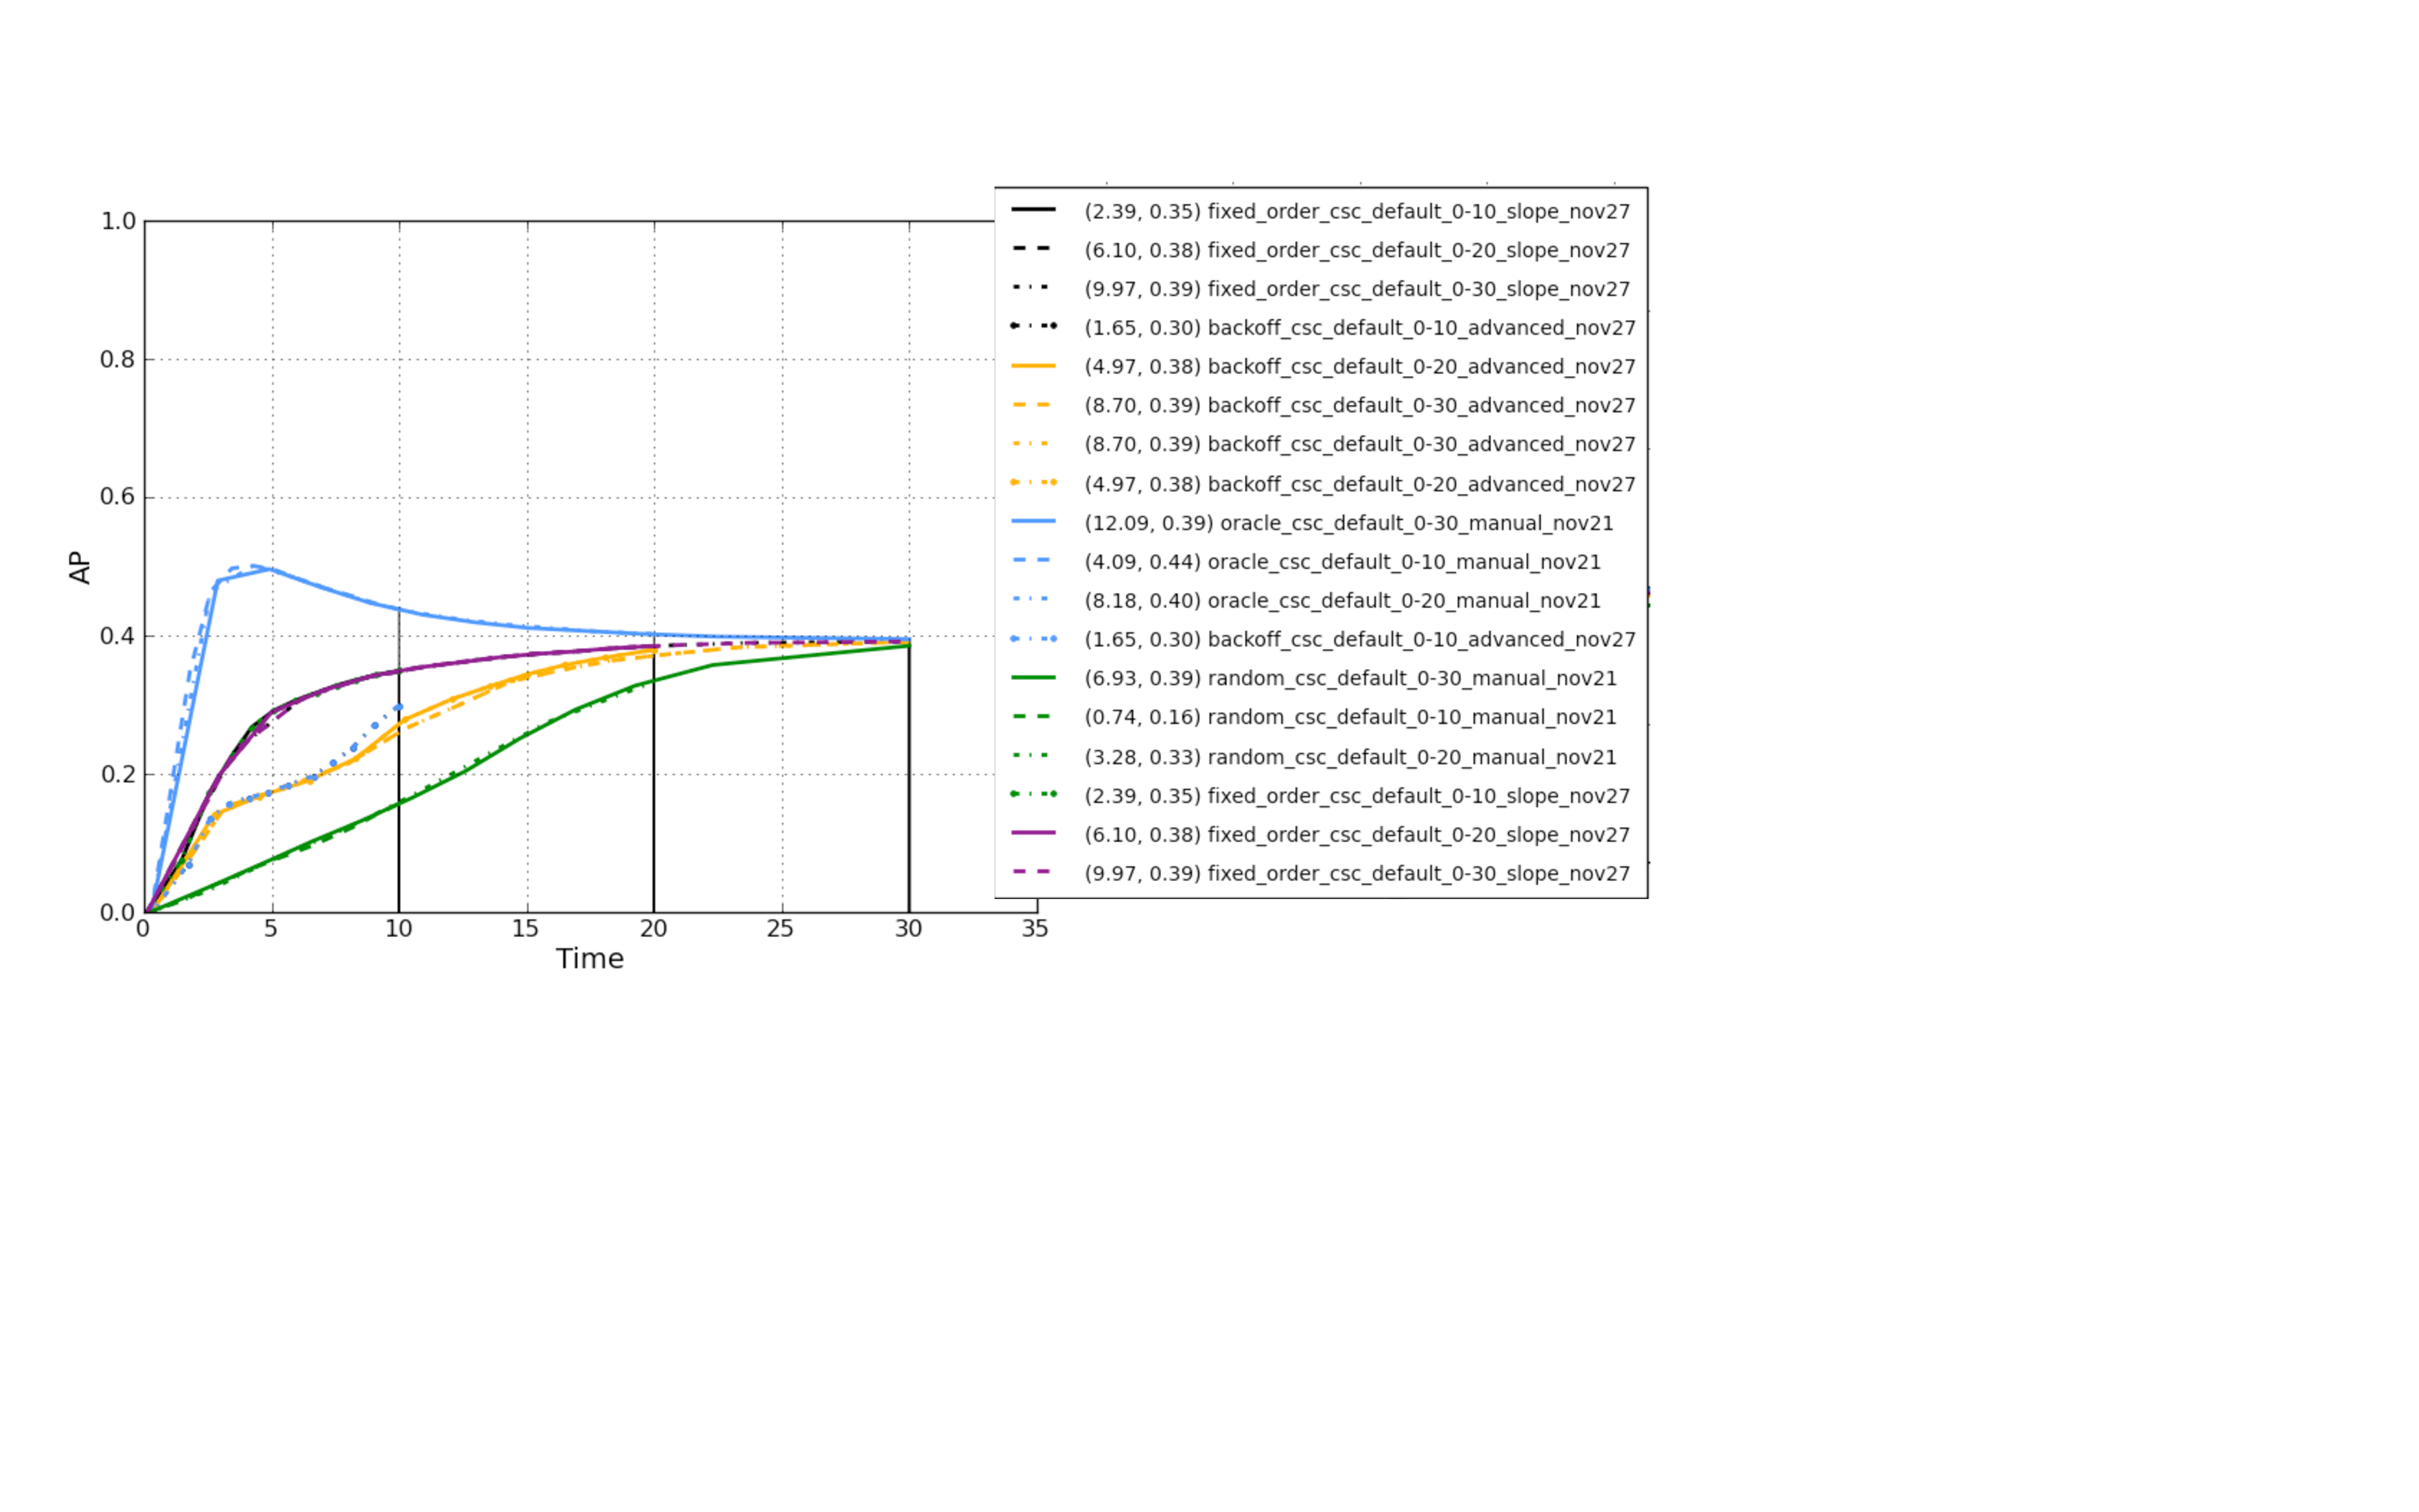
\includegraphics[width=\textwidth]
      {figures/det1.pdf}}
  \caption{\label{fig:1det} The random policy shows the typical path of an uninformed multi-class detector through the image, while the oracle policy shows the room to improve. Our policy results in performance between the two, showing clear improvement over the random baseline.}
\end{figure*}

\section{Policy with multiple detectors per class} \label{sec:multidetector}
We now expand our model to deal with being able to run multiple detectors per class.
We simulate a faster but less robust detector, as would be obtained by modifying the stride or classifier strength, by randomly taking half of the detections output by our base detector, described below in Section \ref{sec:actual-evaluation}.

Simply adding such a detector to the existing system as described would lead to pathological performance.
For example, let's assume that the image contains an object of class 'dog;' we run our most powerful detector for that class and thereafter update our belief state with the strong posterior of this class presence.
Our value function estimates for running the other 'dog' detectors are now increased from before, despite the fact that actually running them is unlikely to produce any new true positives and will in fact probably hurt performance due to false positives.
(Remember that in our evaluation, a ground truth object may only be matched to one detection proposal---all other detections matching that ground truth are considered false positives.)

For this reason, we augment the value function with this consideration.
The only change that needs to be made is to the expected score increase:
\begin{equation}\label{eq:multiclass}
\mathbb{E}[\Delta AP^i] = P(C)\Delta AP^i_{avg} - P(C)\sum_{j \neq i} \delta_j \Delta AP^j_{avg}
\end{equation}
where $\Delta AP^i$ is the score increase of the detector belonging to the action under consideration, the sum is over all other detector actions of the same class as $i$, and $\delta_j$ is an indicator function for whether action $j$ has been taken.

\begin{figure*}[htb]
   \center{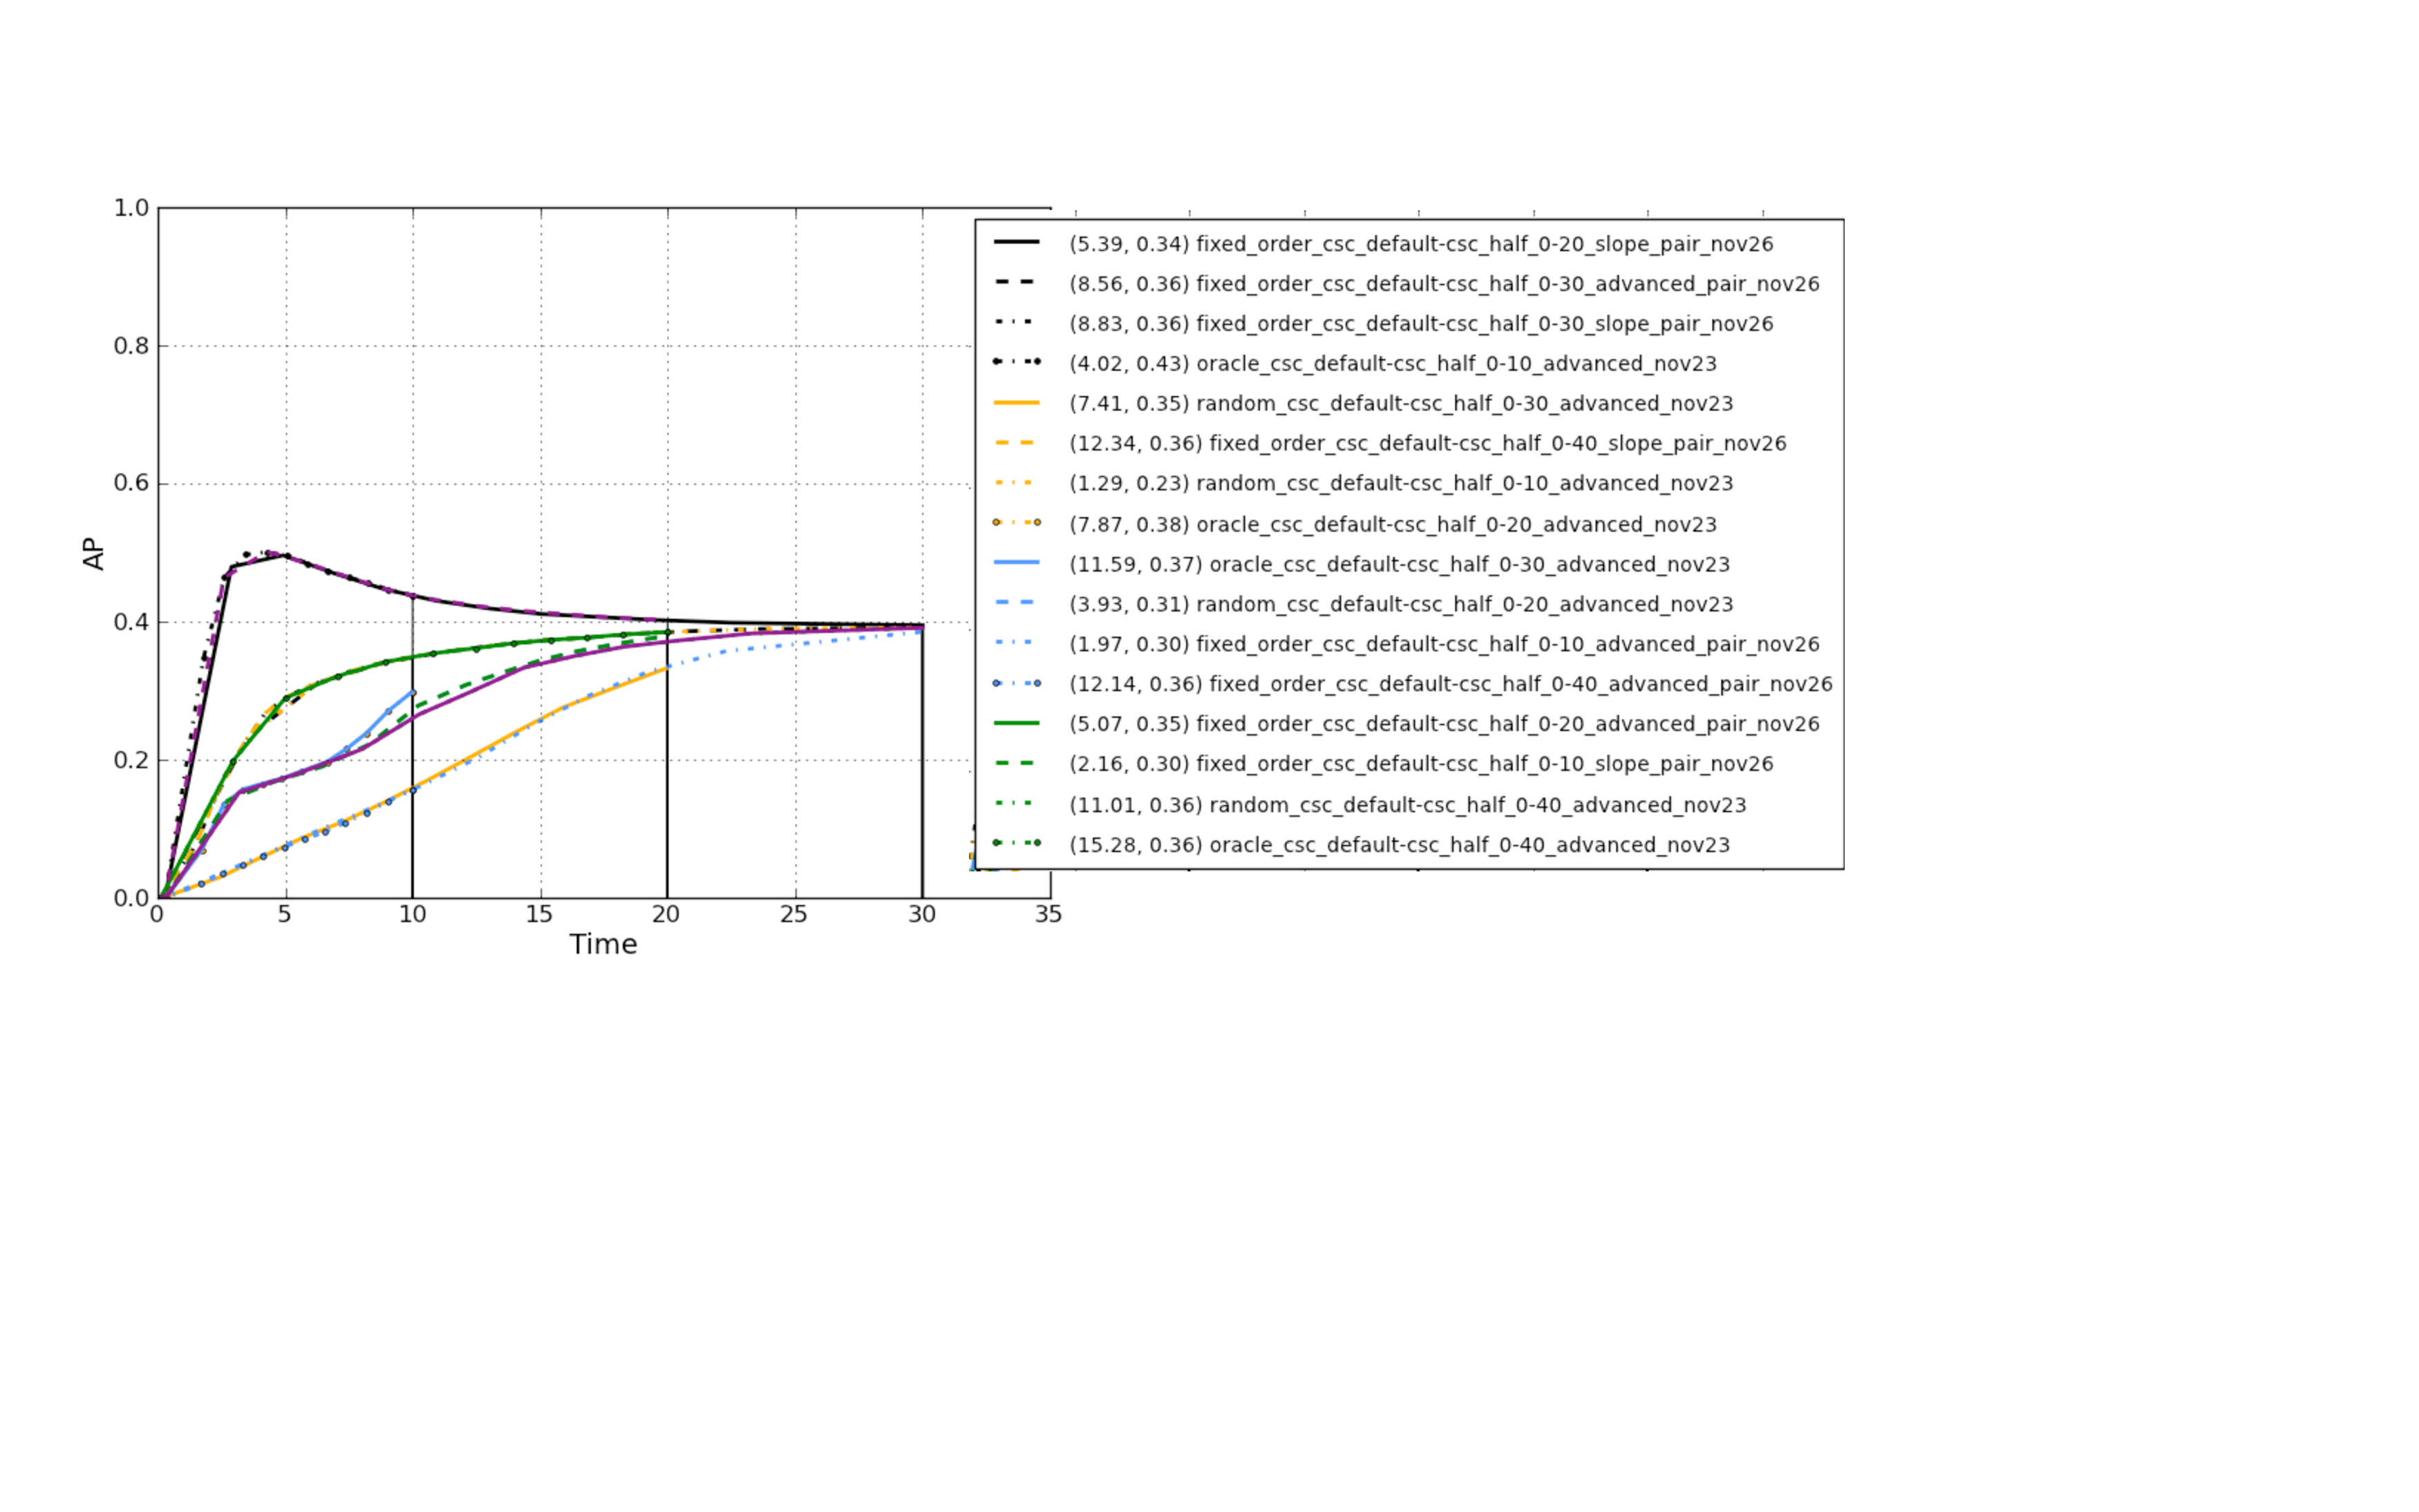
\includegraphics[width=\linewidth]
       {figures/det2.pdf}}
  \caption{\label{fig:2det} When using multiple detectors per class, there is a clear benefit to using a policy that is sensitive to the finite amount of reward that can be obtained from a single class.}
\end{figure*}

Figure \ref{fig:2det} shows the performance comparison of the usual random, oracle, and the two evaluated policies.

Although we do not evaluate this, our system allows for setting priority weights on different detector classes; this results in different policy behaviors.
 % split into sections
\section{Future Work}
\paragraph{Extra-detection actions}
In our implementation of the system, we leave open the possibility of extra-detection actions---those actions that may modify the belief state but not generate any detections directly.
In fact, we implemented one such action: a regression from the GIST \cite{Oliva2001a} feature of the image to object class presence.
In our experiments, this action was always taken first in every policy evaluation; we did not observe an improvement over not using this special action, but leave the question open for further investigation.

\paragraph{Policy Iteration}
While our current implementation shows significant gains over baseline, the gap between our policies' performance and the oracle performance shows that there is yet room to improve.
In particular, we are looking at using the general method of policy iteration to derive approximations of the value function that are able to capture not just greedy but expected rewards to the end of the episode.
Solving POMDPs, of which our stated problem is an example, has not in general been robustly done for problems of this size \cite{Murphy2000,Ng2000}, but there are promising relaxes approaches \cite{Kwok2004}.


\begin{table}
  \begin{center}
    \begin{tabular}{ c| c c c | c }
      Policy & Fixed-order & Backoff & Random & Time\\
      \hline 
       Advanced & 2.17 (0.34) & 1.65 (0.3) & 0.74 & 10 \\
	       & 5.51 (0.38) & 4.97 (0.38) & 3.28 & 20 \\
	       & 9.27 (0.39) & 8.7 (0.39) & 6.93 & 30 \\
      \hline 
      Slope    & 2.39 (0.35) & 2.21 (0.32) & 0.74 & 10 \\
	       & 6.10 (0.38) & 5.76 (0.38) & 3.28 & 20 \\
	       & 9.97 (0.39) & 9.63 (0.39) & 6.93 & 30 \\
      \hline   
      \hline 
      Slope    & 2.16 (0.3) & 1.78 (0.24) &-&10\\
(Double)       & 5.4 (0.34) & 4.24 (0.27) &-&20\\
	       & 8.85 (0.36) & 7.11 (0.32) &-&30\\
	       & 12.36 (0.36) & 10.43 (0.35) &-&40\\
      
      \hline 
      %Double & & & & \\
      \hline 
      Slope    & 2.16 (0.3) & 1.78 (0.24) &-& 10\\
(Pair)         & 5.39 (0.34) & 4.27 (0.27) &-& 20\\
	       & 8.83 (0.36) & 7.22 (0.33) &-& 30\\
	       & 12.34 (0.36) & 10.60 (0.35) &-& 40\\
    \end{tabular}
    \caption{Detailed results of our policies.}
    \label{tab:scoreClassifier}
  \end{center}
\end{table}


{\small
\bibliographystyle{ieee}
\bibliography{../sergeyk-bibtex}
}

\end{document}
